
%% bare_conf.tex
%% V1.4b
%% 2015/08/26
%% by Michael Shell
%% See:
%% http://www.michaelshell.org/
%% for current contact information.
%%
%% This is a skeleton file demonstrating the use of IEEEtran.cls
%% (requires IEEEtran.cls version 1.8b or later) with an IEEE
%% conference paper.
%%
%% Support sites:
%% http://www.michaelshell.org/tex/ieeetran/
%% http://www.ctan.org/pkg/ieeetran
%% and
%% http://www.ieee.org/

%%*************************************************************************
%% Legal Notice:
%% This code is offered as-is without any warranty either expressed or
%% implied; without even the implied warranty of MERCHANTABILITY or
%% FITNESS FOR A PARTICULAR PURPOSE!
%% User assumes all risk.
%% In no event shall the IEEE or any contributor to this code be liable for
%% any damages or losses, including, but not limited to, incidental,
%% consequential, or any other damages, resulting from the use or misuse
%% of any information contained here.
%%
%% All comments are the opinions of their respective authors and are not
%% necessarily endorsed by the IEEE.
%%
%% This work is distributed under the LaTeX Project Public License (LPPL)
%% ( http://www.latex-project.org/ ) version 1.3, and may be freely used,
%% distributed and modified. A copy of the LPPL, version 1.3, is included
%% in the base LaTeX documentation of all distributions of LaTeX released
%% 2003/12/01 or later.
%% Retain all contribution notices and credits.
%% ** Modified files should be clearly indicated as such, including  **
%% ** renaming them and changing author support contact information. **
%%*************************************************************************


% *** Authors should verify (and, if needed, correct) their LaTeX system  ***
% *** with the testflow diagnostic prior to trusting their LaTeX platform ***
% *** with production work. The IEEE's font choices and paper sizes can   ***
% *** trigger bugs that do not appear when using other class files.       ***                          ***
% The testflow support page is at:
% http://www.michaelshell.org/tex/testflow/



\documentclass[conference]{IEEEtran}
% Some Computer Society conferences also require the compsoc mode option,
% but others use the standard conference format.
%
% If IEEEtran.cls has not been installed into the LaTeX system files,
% manually specify the path to it like:
% \documentclass[conference]{../sty/IEEEtran}





% Some very useful LaTeX packages include:
% (uncomment the ones you want to load)


% *** MISC UTILITY PACKAGES ***
%
%\usepackage{ifpdf}
% Heiko Oberdiek's ifpdf.sty is very useful if you need conditional
% compilation based on whether the output is pdf or dvi.
% usage:
% \ifpdf
%   % pdf code
% \else
%   % dvi code
% \fi
% The latest version of ifpdf.sty can be obtained from:
% http://www.ctan.org/pkg/ifpdf
% Also, note that IEEEtran.cls V1.7 and later provides a builtin
% \ifCLASSINFOpdf conditional that works the same way.
% When switching from latex to pdflatex and vice-versa, the compiler may
% have to be run twice to clear warning/error messages.






% *** CITATION PACKAGES ***
%
%\usepackage{cite}
% cite.sty was written by Donald Arseneau
% V1.6 and later of IEEEtran pre-defines the format of the cite.sty package
% \cite{} output to follow that of the IEEE. Loading the cite package will
% result in citation numbers being automatically sorted and properly
% "compressed/ranged". e.g., [1], [9], [2], [7], [5], [6] without using
% cite.sty will become [1], [2], [5]--[7], [9] using cite.sty. cite.sty's
% \cite will automatically add leading space, if needed. Use cite.sty's
% noadjust option (cite.sty V3.8 and later) if you want to turn this off
% such as if a citation ever needs to be enclosed in parenthesis.
% cite.sty is already installed on most LaTeX systems. Be sure and use
% version 5.0 (2009-03-20) and later if using hyperref.sty.
% The latest version can be obtained at:
% http://www.ctan.org/pkg/cite
% The documentation is contained in the cite.sty file itself.






% *** GRAPHICS RELATED PACKAGES ***
%
\ifCLASSINFOpdf
  % \usepackage[pdftex]{graphicx}
  % declare the path(s) where your graphic files are
  % \graphicspath{{../pdf/}{../jpeg/}}
  % and their extensions so you won't have to specify these with
  % every instance of \includegraphics
  % \DeclareGraphicsExtensions{.pdf,.jpeg,.png}
\else
  % or other class option (dvipsone, dvipdf, if not using dvips). graphicx
  % will default to the driver specified in the system graphics.cfg if no
  % driver is specified.
  % \usepackage[dvips]{graphicx}
  % declare the path(s) where your graphic files are
  % \graphicspath{{../eps/}}
  % and their extensions so you won't have to specify these with
  % every instance of \includegraphics
  % \DeclareGraphicsExtensions{.eps}
\fi
% graphicx was written by David Carlisle and Sebastian Rahtz. It is
% required if you want graphics, photos, etc. graphicx.sty is already
% installed on most LaTeX systems. The latest version and documentation
% can be obtained at:
% http://www.ctan.org/pkg/graphicx
% Another good source of documentation is "Using Imported Graphics in
% LaTeX2e" by Keith Reckdahl which can be found at:
% http://www.ctan.org/pkg/epslatex
%
% latex, and pdflatex in dvi mode, support graphics in encapsulated
% postscript (.eps) format. pdflatex in pdf mode supports graphics
% in .pdf, .jpeg, .png and .mps (metapost) formats. Users should ensure
% that all non-photo figures use a vector format (.eps, .pdf, .mps) and
% not a bitmapped formats (.jpeg, .png). The IEEE frowns on bitmapped formats
% which can result in "jaggedy"/blurry rendering of lines and letters as
% well as large increases in file sizes.
%
% You can find documentation about the pdfTeX application at:
% http://www.tug.org/applications/pdftex





% *** MATH PACKAGES ***
%
%\usepackage{amsmath}
% A popular package from the American Mathematical Society that provides
% many useful and powerful commands for dealing with mathematics.
%
% Note that the amsmath package sets \interdisplaylinepenalty to 10000
% thus preventing page breaks from occurring within multiline equations. Use:
%\interdisplaylinepenalty=2500
% after loading amsmath to restore such page breaks as IEEEtran.cls normally
% does. amsmath.sty is already installed on most LaTeX systems. The latest
% version and documentation can be obtained at:
% http://www.ctan.org/pkg/amsmath





% *** SPECIALIZED LIST PACKAGES ***
%
%\usepackage{algorithmic}
% algorithmic.sty was written by Peter Williams and Rogerio Brito.
% This package provides an algorithmic environment fo describing algorithms.
% You can use the algorithmic environment in-text or within a figure
% environment to provide for a floating algorithm. Do NOT use the algorithm
% floating environment provided by algorithm.sty (by the same authors) or
% algorithm2e.sty (by Christophe Fiorio) as the IEEE does not use dedicated
% algorithm float types and packages that provide these will not provide
% correct IEEE style captions. The latest version and documentation of
% algorithmic.sty can be obtained at:
% http://www.ctan.org/pkg/algorithms
% Also of interest may be the (relatively newer and more customizable)
% algorithmicx.sty package by Szasz Janos:
% http://www.ctan.org/pkg/algorithmicx




% *** ALIGNMENT PACKAGES ***
%
%\usepackage{array}
% Frank Mittelbach's and David Carlisle's array.sty patches and improves
% the standard LaTeX2e array and tabular environments to provide better
% appearance and additional user controls. As the default LaTeX2e table
% generation code is lacking to the point of almost being broken with
% respect to the quality of the end results, all users are strongly
% advised to use an enhanced (at the very least that provided by array.sty)
% set of table tools. array.sty is already installed on most systems. The
% latest version and documentation can be obtained at:
% http://www.ctan.org/pkg/array


% IEEEtran contains the IEEEeqnarray family of commands that can be used to
% generate multiline equations as well as matrices, tables, etc., of high
% quality.




% *** SUBFIGURE PACKAGES ***
%\ifCLASSOPTIONcompsoc
%  \usepackage[caption=false,font=normalsize,labelfont=sf,textfont=sf]{subfig}
%\else
%  \usepackage[caption=false,font=footnotesize]{subfig}
%\fi
% subfig.sty, written by Steven Douglas Cochran, is the modern replacement
% for subfigure.sty, the latter of which is no longer maintained and is
% incompatible with some LaTeX packages including fixltx2e. However,
% subfig.sty requires and automatically loads Axel Sommerfeldt's caption.sty
% which will override IEEEtran.cls' handling of captions and this will result
% in non-IEEE style figure/table captions. To prevent this problem, be sure
% and invoke subfig.sty's "caption=false" package option (available since
% subfig.sty version 1.3, 2005/06/28) as this is will preserve IEEEtran.cls
% handling of captions.
% Note that the Computer Society format requires a larger sans serif font
% than the serif footnote size font used in traditional IEEE formatting
% and thus the need to invoke different subfig.sty package options depending
% on whether compsoc mode has been enabled.
%
% The latest version and documentation of subfig.sty can be obtained at:
% http://www.ctan.org/pkg/subfig




% *** FLOAT PACKAGES ***
%
%\usepackage{fixltx2e}
% fixltx2e, the successor to the earlier fix2col.sty, was written by
% Frank Mittelbach and David Carlisle. This package corrects a few problems
% in the LaTeX2e kernel, the most notable of which is that in current
% LaTeX2e releases, the ordering of single and double column floats is not
% guaranteed to be preserved. Thus, an unpatched LaTeX2e can allow a
% single column figure to be placed prior to an earlier double column
% figure.
% Be aware that LaTeX2e kernels dated 2015 and later have fixltx2e.sty's
% corrections already built into the system in which case a warning will
% be issued if an attempt is made to load fixltx2e.sty as it is no longer
% needed.
% The latest version and documentation can be found at:
% http://www.ctan.org/pkg/fixltx2e


%\usepackage{stfloats}
% stfloats.sty was written by Sigitas Tolusis. This package gives LaTeX2e
% the ability to do double column floats at the bottom of the page as well
% as the top. (e.g., "\begin{figure*}[!b]" is not normally possible in
% LaTeX2e). It also provides a command:
%\fnbelowfloat
% to enable the placement of footnotes below bottom floats (the standard
% LaTeX2e kernel puts them above bottom floats). This is an invasive package
% which rewrites many portions of the LaTeX2e float routines. It may not work
% with other packages that modify the LaTeX2e float routines. The latest
% version and documentation can be obtained at:
% http://www.ctan.org/pkg/stfloats
% Do not use the stfloats baselinefloat ability as the IEEE does not allow
% \baselineskip to stretch. Authors submitting work to the IEEE should note
% that the IEEE rarely uses double column equations and that authors should try
% to avoid such use. Do not be tempted to use the cuted.sty or midfloat.sty
% packages (also by Sigitas Tolusis) as the IEEE does not format its papers in
% such ways.
% Do not attempt to use stfloats with fixltx2e as they are incompatible.
% Instead, use Morten Hogholm'a dblfloatfix which combines the features
% of both fixltx2e and stfloats:
%
% \usepackage{dblfloatfix}
% The latest version can be found at:
% http://www.ctan.org/pkg/dblfloatfix




% *** PDF, URL AND HYPERLINK PACKAGES ***
%
%\usepackage{url}
% url.sty was written by Donald Arseneau. It provides better support for
% handling and breaking URLs. url.sty is already installed on most LaTeX
% systems. The latest version and documentation can be obtained at:
% http://www.ctan.org/pkg/url
% Basically, \url{my_url_here}.



% *** Do not adjust lengths that control margins, column widths, etc. ***
% *** Do not use packages that alter fonts (such as pslatex).         ***
% There should be no need to do such things with IEEEtran.cls V1.6 and later.
% (Unless specifically asked to do so by the journal or conference you plan
% to submit to, of course. )

\usepackage{graphicx}
\usepackage{float}
\usepackage{listings}
% correct bad hyphenation here
\hyphenation{op-tical net-works semi-conduc-tor}


\begin{document}
%
% paper title
% Titles are generally capitalized except for words such as a, an, and, as,
% at, but, by, for, in, nor, of, on, or, the, to and up, which are usually
% not capitalized unless they are the first or last word of the title.
% Linebreaks \\ can be used within to get better formatting as desired.
% Do not put math or special symbols in the title.
\title{DiskSim Project\\ Week Three}


% author names and affiliations
% use a multiple column layout for up to three different
% affiliations
\author{\IEEEauthorblockN{Jiafei Song}
\IEEEauthorblockA{School of Information and\\Science Technology\\
songjf@shanghaitech.edu.cn\\
ShanghaiTech University}
\and
\IEEEauthorblockN{Yuan Yuan}
\IEEEauthorblockA{School of Information and\\Science Technology\\
yuanyuan1@shanghaitech.edu.cn\\
ShanghaiTech University}
\and
\IEEEauthorblockN{Yusen Lin}
\IEEEauthorblockA{School of Information and\\Science Technology\\
linys@shanghaitech.edu.cn\\
ShanghaiTech University}}

% conference papers do not typically use \thanks and this command
% is locked out in conference mode. If really needed, such as for
% the acknowledgment of grants, issue a \IEEEoverridecommandlockouts
% after \documentclass

% for over three affiliations, or if they all won't fit within the width
% of the page, use this alternative format:
%
%\author{\IEEEauthorblockN{Michael Shell\IEEEauthorrefmark{1},
%Homer Simpson\IEEEauthorrefmark{2},
%James Kirk\IEEEauthorrefmark{3},
%Montgomery Scott\IEEEauthorrefmark{3} and
%Eldon Tyrell\IEEEauthorrefmark{4}}
%\IEEEauthorblockA{\IEEEauthorrefmark{1}School of Electrical and Computer Engineering\\
%Georgia Institute of Technology,
%Atlanta, Georgia 30332--0250\\ Email: see http://www.michaelshell.org/contact.html}
%\IEEEauthorblockA{\IEEEauthorrefmark{2}Twentieth Century Fox, Springfield, USA\\
%Email: homer@thesimpsons.com}
%\IEEEauthorblockA{\IEEEauthorrefmark{3}Starfleet Academy, San Francisco, California 96678-2391\\
%Telephone: (800) 555--1212, Fax: (888) 555--1212}
%\IEEEauthorblockA{\IEEEauthorrefmark{4}Tyrell Inc., 123 Replicant Street, Los Angeles, California 90210--4321}}




% use for special paper notices
%\IEEEspecialpapernotice{(Invited Paper)}




% make the title area
\maketitle

% As a general rule, do not put math, special symbols or citations
% in the abstract
\begin{abstract}
This project is to have a better understanding of storage systems with the tool of DiskSim,especially disk storage systems. And the whole project will be divided into four parts to complete.
\end{abstract}

% no keywords




% For peer review papers, you can put extra information on the cover
% page as needed:
% \ifCLASSOPTIONpeerreview
% \begin{center} \bfseries EDICS Category: 3-BBND \end{center}
% \fi
%
% For peerreview papers, this IEEEtran command inserts a page break and
% creates the second title. It will be ignored for other modes.
\IEEEpeerreviewmaketitle



\section{\emph{\textbf{Overview}}}
% no \IEEEPARstart
DiskSim is an efficient, accurate, highly-configurable disk system simulator originally developed at the University of Michigan and enhanced at CMU to support research into various aspects of storage subsystem architecture.

\subsection{\emph{\textbf{Background}}}
It is written in C and requires no special system software (just basic POSIX interfaces). DiskSim includes modules for most secondary storage components of interest, including device drivers, buses, controllers, adapters, and disk drives. DiskSim also includes support for a number of externally-provided trace formats and internally-generated synthetic workloads, and includes hooks for inclusion in a larger scale system-level simulator.
\subsection{\emph{\textbf{Usage}}}
It has been used in a variety of published studies (and several unpublished studies) to understand modern storage subsystem, to understand how storage performance relates to overall system, and to evaluate new storage subsystem.
\subsection{\emph{\textbf{Structure}}}
There are two main executable file in the whole system . One is Disksim.c and another is Syssim\underline{ }driver.c.
\subsubsection{\emph{\textbf{Disksim}}}
There are five parameters for this function, including the: parfile,outfile,tracetype,tracefile,synthgen.\\
\textbf{\emph{Parfile:}}aka parameter file. DiskSim can be configured via the parameter file to model a wide variety of storage subsystems. It uses libparam to input the parameter file.\\
\textbf{\emph{Outfile:}}The output of simulation. It can be modified by the parameter file.\\
\textbf{\emph{Tracetype:}}The type of trace file. ASCII, HPL, HPL2, DEC, RAW, VALIDATE, EMCSYMM, DEFAULT(ASCII) and so on. You can also add new type.\\
\textbf{\emph{Tracefile:}}The format of the tracefile is request arrival time, device number, block number, request size, request flags. Zero means generating data by parameter file.If it's zero, synthegen must be larger then zero.\\
\textbf{\emph{synthgen:}}The value of synthgen means how many generators used to get trace, one generator represents a process to generator input.\\


\subsubsection{\emph{\textbf{Syssim\underline{ }driver}}}
\begin{flushleft}
\quad
disksim provides disksim\underline{ }interface.c to make disksim as  subsystem to get result by external requests . And this function is to use this interface to simulate the disk.
\end{flushleft}

\section{\emph{\textbf{Case Study}}}
\subsection{\emph{\textbf{Configuration and Installation}}}
\begin{flushleft}
\quad We run DiskSim-4.0 on 32-bit Ubuntu 14.04 LTS.\\
\quad 1) Download disksim-4.0.tar.gz from http://www.pdl.cmu.edu/DiskSim/ \\
\quad 2) Run the commands $ tar xfz disksim-4.0.tar.gz $ and $cd disksim-4.0$ in the terminal.\\
\quad 3) In $memsmodel/Makefile$, \\
\quad \textbf{repalce}\\
\quad \quad ems\_seektest: mems\_seektest.o libmems\_internals.a \$(CC) -o \$@ mems\_seektest.o \$(LDFLAGS) \$(CFLAGS) -lmems\_internals \\
\quad \textbf{with}\\
\quad \quad ems\_seektest: mems\_seektest.o libmems\_internals.a \$(CC) -o \$@ mems\_seektest.o \$(CFLAGS) -lmems\_internals \$(LDFLAGS) \\
\quad 4) In $src/Makefile$, \\
\quad \textbf{repalce}\\
\quad \quad LDFLAGS = -lm -L. -ldisksim \$(DISKMODEL\_LDFLAGS) \$(MEMSMODEL\_LDFLAGS) \$(LIBPARAM\_LDFLAGS) \$(LIBDDBG\_LDFLAGS) \\
\quad \textbf{with}\\
\quad \quad LDFLAGS = -L. -ldisksim \$(DISKMODEL\_LDFLAGS) \$(MEMSMODEL\_LDFLAGS) \$(LIBPARAM\_LDFLAGS) \$(LIBDDBG\_LDFLAGS) -lm \\
\quad 5) Run the command $make$ in the terminal. \\
\quad 6) Run the command $cd valid; ./runvalid$ in the terminal. \\
\end{flushleft}
\subsection{\emph{\textbf{Parameter initialize}}}
\begin{flushleft}
    In the disksim\underline{ }logorg org0:\\
    \quad Addressing Mode = Array\\
    \quad Distribution scheme = Striped\\
    \quad Redundancy scheme = Striped\\
    \quad devices = [disk0..disk8]\\
    In the disksim\underline{ }synthio Synthio:\\
    change distribution to normal
\end{flushleft}
\subsection{\emph{\textbf{Run}}}
\begin{flushleft}
  In the valid folder, run:
\end{flushleft}
   ../src/disksim synthraid0.parv synthraid0.outv ascii 0 1\\
   grep "IOdriver Response time average" synthraid0.outv

\subsection{\emph{\textbf{Result:}}}
\begin{flushleft}
  IOdriver Response time average : 19.438945
\end{flushleft}

\section{\emph{\textbf{Raid5}}}
\subsection{\emph{\textbf{Parameter initialize}}}
\begin{flushleft}
\#component instantiation \\
instantiate [ statfoo ] as Stats\\
instantiate [ ctlr0 .. ctlr4 ] as CTLR0\\
instantiate [ bus0 ] as BUS0\\
instantiate [ disk0 .. disk4 ] as HP\underline{ }C3323A\\
instantiate [ driver0 ] as DRIVER0\\
instantiate [ bus1 .. bus5 ] as BUS1\\
\quad \\\quad  \\
disksim\underline{ }logorg org0\{\\
\quad Addressing mode = Array \\
\quad Distribution scheme = Striped \\
\quad Redundancy scheme = Parity\underline( )rotated \\
\quad devices = [ disk0 .. disk4 ]\\
\quad ...\\
\}\\
\quad \\
disksim\underline{ }synthgen\{ \# generator0 \\
\quad Storage capacity per device  =  8224032\\
\quad  devices = [ org0 ],\\
\quad       Blocking factor =  8,\\
\quad       Probability of sequential access =  0.2,\\
\quad       Probability of local access =  0.4,\\
\quad       Probability of read access =  0.66,\\
\quad       Probability of time-critical request =  0.1,\\
\quad       Probability of time-limited request =  0.3,\\
\quad       Time-limited think times  = [ normal, 30.0, 100.0  ],\\
\quad       General inter-arrival times  = [ exponential, 0.0, 10.0  ],\\
\quad       Sequential inter-arrival times  = [ exponential, 0.0, 10.0  ],\\
\quad       Local inter-arrival times  = [ exponential, 0.0, 10.0  ],\\
\quad       Local distances  = [ normal, 0.0, 40000.0  ],\\
\quad       Sizes  = [ exponential, 0.0, 8.0  ]\\
\} \# end of generator 0  \\
\quad \\
PS. In this part, we particularly use 5 disks to do the simulation.
\end{flushleft}
\subsection{\emph{\textbf{Result}}}



\begin{figure}[H]
  \centering
  % Requires \usepackage{graphicx}
  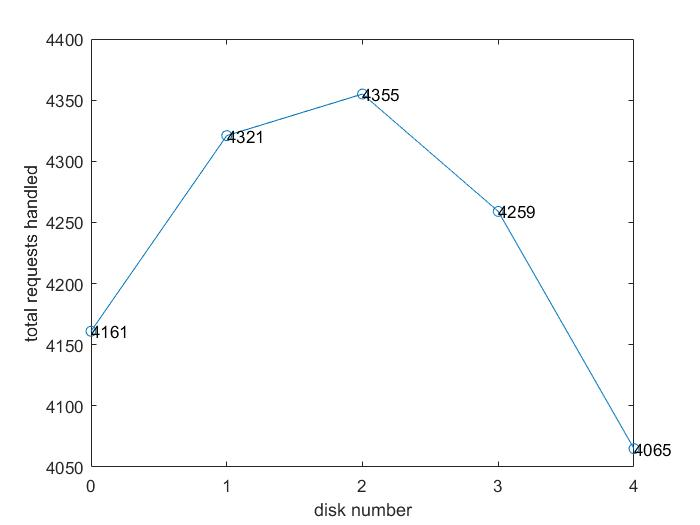
\includegraphics[width=3.4in]{request.jpg}\\
  \caption{disk id vs total requests handled}\label{figure1}
\end{figure}
\begin{figure}[H]
  \centering
  % Requires \usepackage{graphicx}
  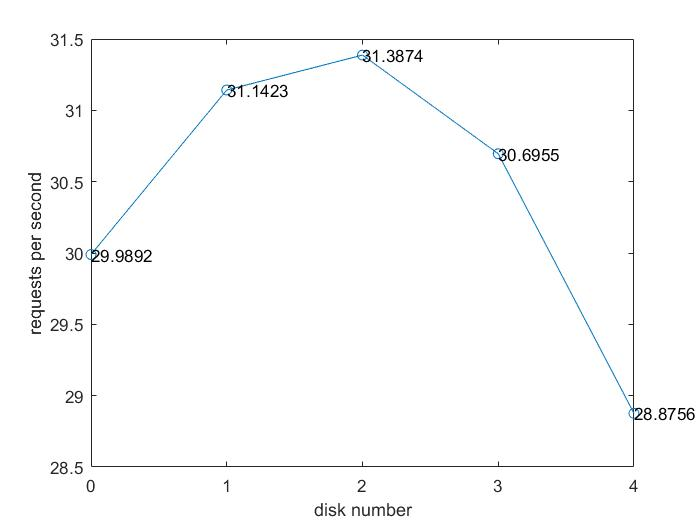
\includegraphics[width=3.4in]{request_per.jpg}\\
  \caption{disk id vs requests per second}\label{figure2}
\end{figure}
\begin{figure}[H]
  \centering
  % Requires \usepackage{graphicx}
  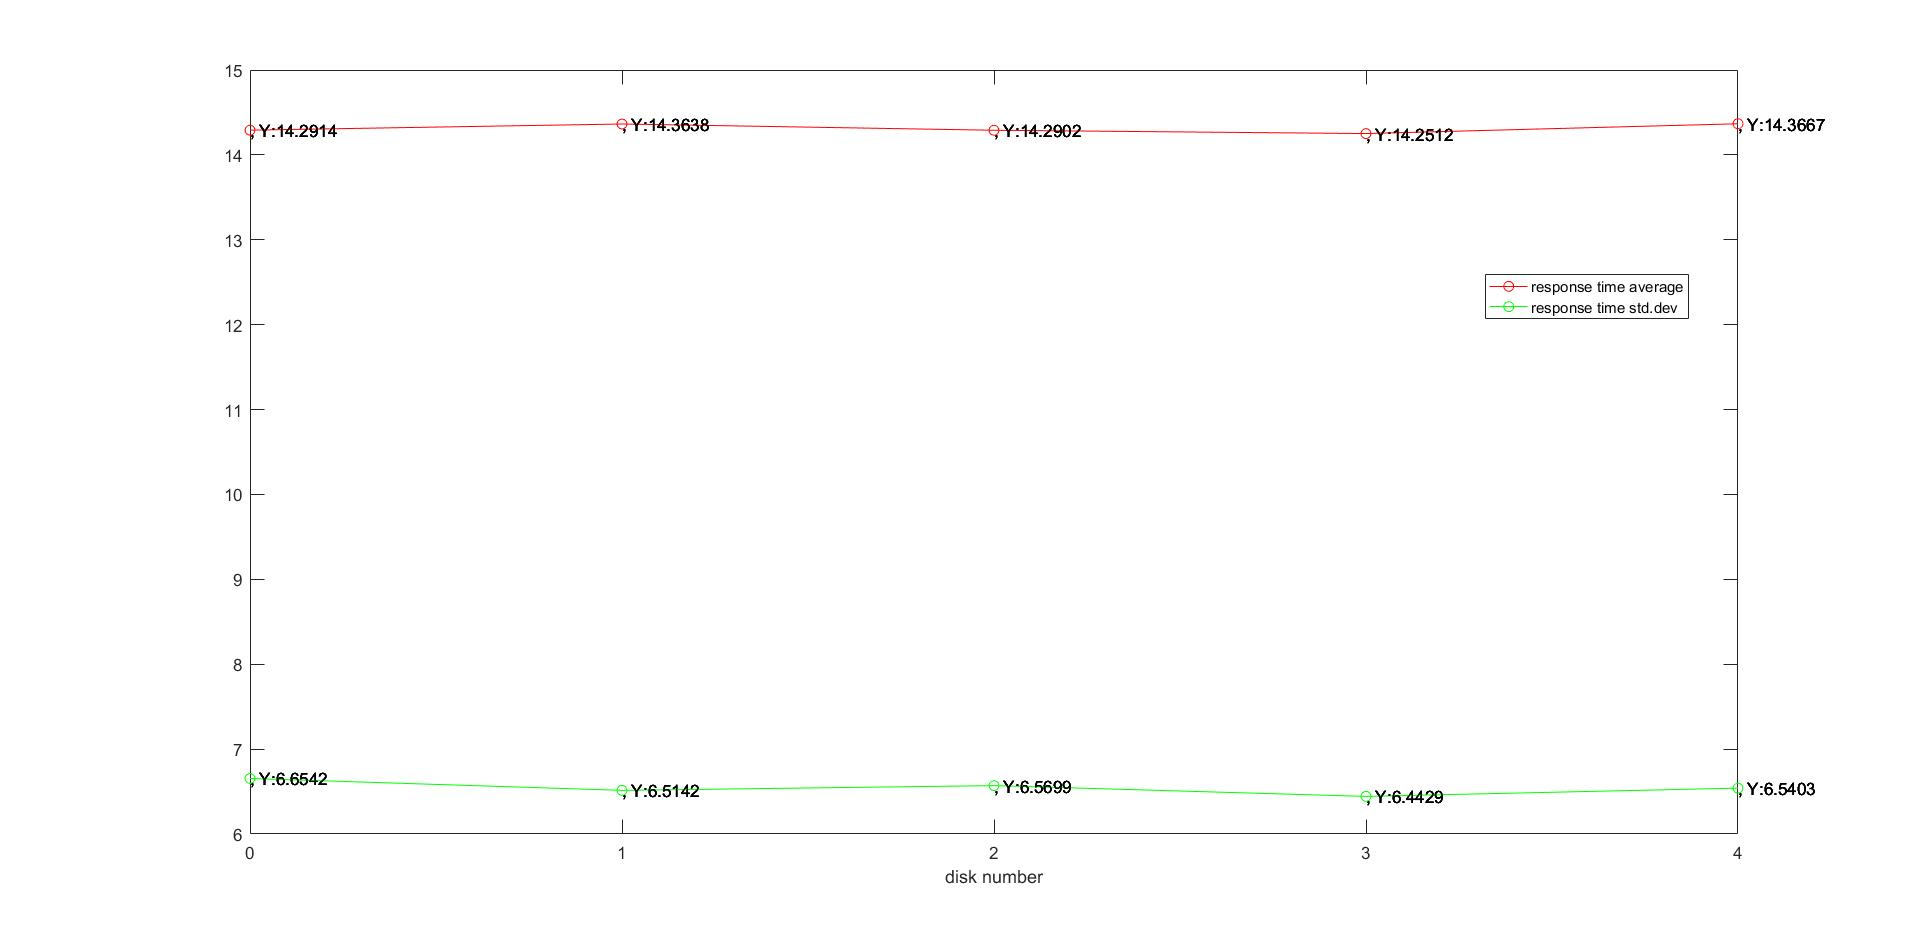
\includegraphics[width=3.4in]{result.jpg}\\
  \caption{disk id vs response time}\label{figure3}
\end{figure}
\begin{figure}[H]
  \centering
  % Requires \usepackage{graphicx}
  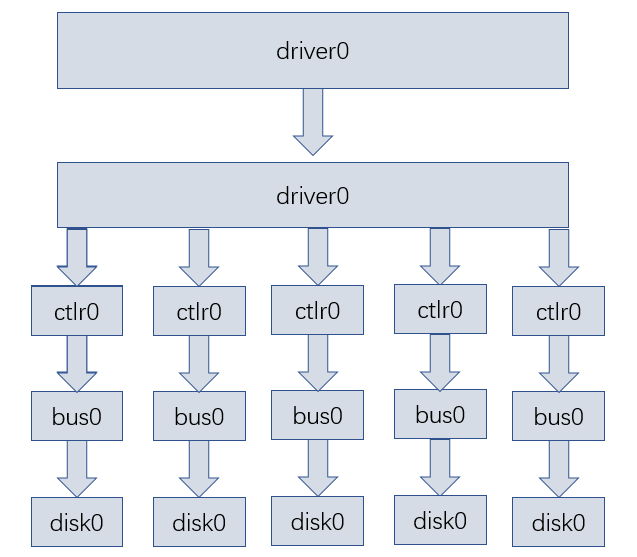
\includegraphics[width=3.4in]{topo.png}\\
  \caption{topology of raid5-5}\label{figure4}
\end{figure}


\section{\emph{\textbf{PARAID5}}}
\subsection{\emph{\textbf{Parameter initialize}}}
There are gears: one with 4 disks (gear 1) and the other with 5 disks (gear 2).Each gear has its own parameter file.The parameter file of the one with 5 disks is the same with that of the 5-disk RAID-5.\\
We made the following change in that of 4-disk one.\\
1)  [ ctlr0 .. ctlr4 ] ----$>$  [ ctlr0 .. ctlr3 ]\\
2) [ disk0 .. disk4 ] ----$>$ [ disk0 .. disk3 ]\\
3) Storage capacity per device  =  8224032  ----$>$ Storage capacity per device  =  6168024\\
\subsection{\emph{\textbf{Implementation}}}
We call the parameter file of gear 1 "paraid5\_1.parv" and out file "paraid5\_1.outv". We call the parameter file of gear 2 "paraid5\_2.parv" and out file "paraid5\_2.outv". We write a python code to transfer from one gear to the other. To run command line in python, we use the os package.\\
For example,
\lstset{flexiblecolumns,showstringspaces=false,numbers=left,numberstyle=\footnotesize,frame=single,breaklines=ture}
\begin{lstlisting}[language=Python]
import os
os.system("ls -l")
\end{lstlisting}
will show the detailed file information in the current route, which just like call "ls -l" in the terminal.\\
By running
\begin{lstlisting}[language=Python]
os.system("../src/disksim paraid5_1.parv paraid5_1.outv ascii 0 1")
\end{lstlisting}
we get paraid5\_1.outv. The srcipt will open the outv file and read it line by line. It search for the line with string "Completely idle time:" at the location of [8:29]. For example, the line may be "Disk \#1 Completely idle time:  	15059.014877   	0.470399". We split the line and get the last part as the idle time ratio. We regard $1-idle\ time\ ratio$ as utilization time ratio. U denotes the average of the utilization time ratios of the disks and S denotes the stand deviation of utilization time.\\
What we do in gear 2 is similar.\\
When in gear 1, if $U+S>T$, shift up. When in gear 2, if $U+S<T$, shift down.\\
The python code runs the disksim 8 times to simulate 8 time windows. After each time window, it checks if $U+S>T$ or $U+S<T$. Then it will shift up or shift down if needed.
\subsection{\emph{\textbf{Result}}}
In our test,the result is the following.\\
\begin{table}[H]
\centering
\begin{tabular}{ccccc}
\hline
gear		&disks		&U			&S 					&U+S			\\ \hline
1			&4			&0.5094005	&0.0463932240568 	&0.555793724057	\\ \hline
2			&5			&0.4321564	&0.0251287172503	&0.45728511725	\\ \hline
\end{tabular}
\caption{U and S for each gear}
\end{table}
We set threshold T to 0.8.
\begin{figure}[H]
  \centering
  % Requires \usepackage{graphicx}
  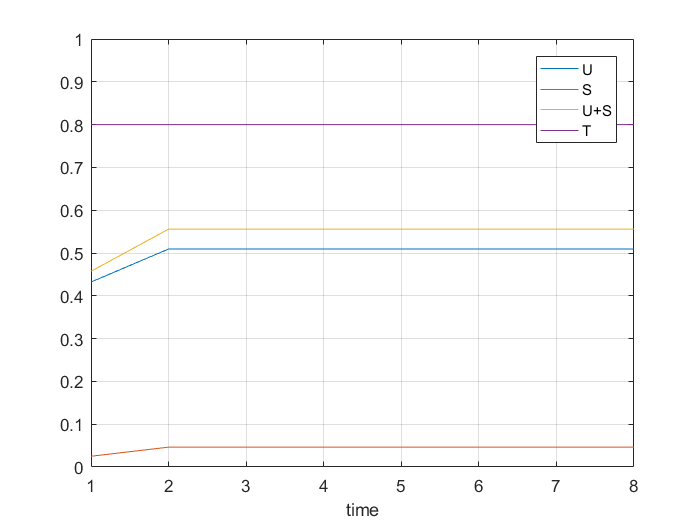
\includegraphics[width=4in]{utilization.png}\\
  \caption{U,S,U+S,T vs time}\label{figure2}
\end{figure}
At first, it is in gear 2. Since $U+S<T$, it shifts down and then levels out at gear 1.
\subsection{\emph{\textbf{Theory Analysis}}}
Gearing is a process of drving a car. If we want to change the drving mode, we need gear. Gearing of the PARAID is similar to gearing of the car.\\

There are three modes of disks: idle, standby and active. Certainly,the active mode consumes more energy than other modes. However, switching mode also consumes lots of energy. To save energy, we need keep balance among the modes.\\

An idea is that we let fewer disks respond to the I/O instructions when the total workload is not heavy and let more disks respond to the I/O instructions when the total workload is heavy. Hence the workload is asymmetric. PARAID works in this way.\\
\subsection{\emph{\textbf{Difficulties}}}
It's very difficult and we just made a naive version. What we can do is reading the DiskSim Manual[1] and "PARAID" paper[2]. Perhaps we need more guidance from teacher and TAs.



% trigger a \newpage just before the given reference
% number - used to balance the columns on the last page
% adjust value as needed - may need to be readjusted if
% the document is modified later
%\IEEEtriggeratref{8}
% The "triggered" command can be changed if desired:
%\IEEEtriggercmd{\enlargethispage{-5in}}

% references section

% can use a bibliography generated by BibTeX as a .bbl file
% BibTeX documentation can be easily obtained at:
% http://mirror.ctan.org/biblio/bibtex/contrib/doc/
% The IEEEtran BibTeX style support page is at:
% http://www.michaelshell.org/tex/ieeetran/bibtex/
%\bibliographystyle{IEEEtran}
% argument is your BibTeX string definitions and bibliography database(s)
%\bibliography{IEEEabrv,../bib/paper}
%
% <OR> manually copy in the resultant .bbl file
% set second argument of \begin to the number of references
% (used to reserve space for the reference number labels box)

\subsection{\emph{\textbf{Analysis and Implement in Source Code}}}
\begin{flushleft}
  main() defined  in disksim\underline{ }main.c \\
  disksim\underline{ }run\underline{ }simulation() defined in disksim.c\\
  disksim\underline{ }simlulate\underline{ }event() defined in disksim.c\\
  io\underline{ }internal\underline{ }event() defined in disksim\underline{ }iosim.c\\
  iodriver\underline{ }request() defined in disksim\underline{ }iodriver.c \\
  logorg\underline{ }maprequest() defined in disksim\underline{ }logorg.c \\
  logorg\underline{ }parity\underline{ }table() defined in disksim\underline{ }redun.c\\
\subsubsection{\textbf{Gear Shifting condition}}
    \begin{flushleft}
\quad      Up-shifts: U+S $>$ T \\
\quad      U: average utilization of disks\\
\quad      S: standard deviation of U\\
\quad      U = (total\underline{ }time - idle\underline{ }time)/total\underline{ }time
    \end{flushleft}
\subsubsection{\textbf{Remapping}}
    \begin{flushleft}
\quad   In this part,we do not implement it completely.\\
\quad   Each request is represented as a structure,contains device number , block number and so on.\\
\quad   All the requests are organized as a linked list,so that we can track back to reassign the number of each request.\\
\quad   The request is defined in disksim\underline{ }global.c named ioreq\underline{ }event.\\
    \end{flushleft}
\end{flushleft}

\section{\emph{\textbf{Power Management Module}}}
\subsection{\emph{\textbf{Parameters Initialize}}}
To calculate the power consumption of PARAID-5, we need to know the power of each disk and the utilization time of each disk, maybe as well as the gear switching energy but here we just neglect it.Here we define the power of each disk is 14.2.\\
\subsection{\emph{\textbf{Results and Comparations}}}
Running our python program before, we get detailed information about utilization time of each period.\\
\begin{lstlisting}
gear 2: 5 disk
IOdriver Response time average:         24.303764
average utilization time: 0.4321564
stand deviation of utilization time: 0.0251287172503
U+S= 0.45728511725
>>>>>>>>
U+S<T, should down-shift.

gear 1: 4 disk
IOdriver Response time average:         27.285464
average utilization time: 0.5094005
stand deviation of utilization time: 0.0463932240568
U+S= 0.555793724057
>>>>>>>>
U+S<T, don't need to up-shift.

......

\end{lstlisting}
And we use a table to represent what we need.
\begin{table}[H]
\centering
\begin{tabular}{ccccc}
\hline
gear		&disks		&U			&P 					&U*P*disks			\\ \hline
1			&4			&0.5094005	&14.2 	&28.9339484	\\ \hline
2			&5			&0.4321564	&14.2 	&30.6831044	\\ \hline
\end{tabular}
\caption{U*P*disks is power consumption}
\end{table}
\begin{figure}[H]
  \centering
  % Requires \usepackage{graphicx}
  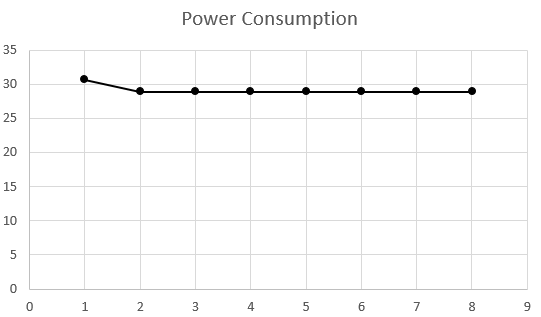
\includegraphics[width=4in]{result2.png}\\
  \caption{Power consumption vs time}\label{figure3}
\end{figure}
By gear shifting from 5-disk to 4-disk, about 5.7 percent of energy is preserved.
\subsection{\emph{\textbf{Theory Analysis}}}
    \begin{flushleft}
\quad   PARAID-5 is designed to save more energy while remain similar performance compared with RAID5. RAID5 is configued for peak performance and it keeps all disks spinning for light loads. In this case, there are two parts can be paid attention to decrease power consumtion.One is unused storage capacity caused by over-provision of storage capacity and unused storage can be traded for energy savings.Another is fluctuating load caused by frequent on-off power transitions.\\
\quad   According to what mentioned above, PARAID-5 uses group of disks of differnent size to form gears. The design of gears organized into hierarchical overlapping subsets and can utilize over-provisioned spare storage in RAID.When operating in small gear, other disks are powered off.To decide the shifting of gears, the workload should be approximated and gear shift into most appropriate gear, in order to minimize the opportunity lost to save power.The shift of gear is controlled by utilization time and stand deviation of it, which is detailed explained above.The disign is useful to adapt cyclic fluctuating workload.\\
\quad   Because of these kind of designs, PARAID can preserve energy.But how can it maintains a acceptable peroformance? Three ways should be used to achieve the goal. First, PARAID operate in the highest gear when the system demands peak performance and uses the same disk layout. Second, maximize parallelism within each gear. Third, delay block replication until gear shifting.Though our PARAID has only two gears, using three or more gears is of better performance in reality.Then disks can be divided into three types: busy disks(in all gears), standby disks(in gears exclude lower gears), and idle disks(in higher gears).Role exchange between outside disks with middle disks can maintain reliability.
    \end{flushleft}

\subsection{\emph{\textbf{Difficulties}}}
It's too difficult that we even wasted many days reading everything can be searched about this mission but get little help. And after asking some people, we simply made a naive version and we found it difficult to understand all the theory behind it. Actually we hope to read some recommended papers from teacher and TAs. 

% trigger a \newpage just before the given reference
% number - used to balance the columns on the last page
% adjust value as needed - may need to be readjusted if
% the document is modified later
%\IEEEtriggeratref{8}
% The "triggered" command can be changed if desired:
%\IEEEtriggercmd{\enlargethispage{-5in}}

% references section

% can use a bibliography generated by BibTeX as a .bbl file
% BibTeX documentation can be easily obtained at:
% http://mirror.ctan.org/biblio/bibtex/contrib/doc/
% The IEEEtran BibTeX style support page is at:
% http://www.michaelshell.org/tex/ieeetran/bibtex/
%\bibliographystyle{IEEEtran}
% argument is your BibTeX string definitions and bibliography database(s)
%\bibliography{IEEEabrv,../bib/paper}
%
% <OR> manually copy in the resultant .bbl file
% set second argument of \begin to the number of references
% (used to reserve space for the reference number labels box)
\begin{thebibliography}{1}

\bibitem{IEEEhowto:kopka}
    DiskSim Version 4.0 Reference Manual: http://www.pdl.cmu.edu/PDL-FTP/DriveChar/CMU-PDL-08-101.pdf
\bibitem{IEEEhowto:kopka}
	Weddle, Charles, et al. "PARAID: The gearshifting power-aware RAID." Acm Transactions on Storage 3.3(2007):13.
\end{thebibliography}




% that's all folks
\end{document}


